\chapter{Predicting who is next: the cascade model}
\label{ch:cascade}

\section{The idea}
\begin{simplebox}
Once a service is in trouble, the interesting question for the engineer is: \emph{who else is about to be hurt?} Not every dependency passes trouble along. A service with a timeout, a cache or a circuit breaker may shrug off a failing dependency. A service with none of those may collapse right away. We cannot read the code to find out which is which, so we \emph{learn it from experience}: every time one service goes bad, we look at the services that call it and ask, within a minute, did they go bad too? Over time each connection collects a track record, like ``this link has passed trouble along 6 times out of 8''.
\end{simplebox}

\begin{techbox}
Each call edge $c\to x$ carries an unknown probability $p(c\leftarrow x)$ that trouble in $x$ reaches its caller $c$. Whenever a service $x$ turns abnormal, every healthy caller $c$ is one \emph{trial}; it succeeds if $c$ turns abnormal within one minute (12 windows). With $k$ successes in $n$ trials and a Beta prior of mean $\pi_0$ and strength $m$, the posterior mean is
\[
\hat p(c\leftarrow x)=\frac{k+m\,\pi_0}{n+m}.
\]
All experiments use an uninformative prior ($\pi_0=0.5$, $m=2$). No labels are needed: the trials are the system's own history.
\end{techbox}

\begin{examplebox}[Worked example: one edge's track record]
Prior: mean $0.5$, strength $2$ (so it behaves like having seen 1 success and 1 failure). The edge \code{orders}$\leftarrow$\code{orders-db}.

\begin{center}
\small
\begin{tabular}{lcc}
\toprule
After & $k/n$ & $\hat p=(k+1)/(n+2)$\\
\midrule
no trials & 0/0 & $1/2=0.50$\\
1 trial, success & 1/1 & $2/3=0.67$\\
3 trials, 3 successes & 3/3 & $4/5=0.80$\\
8 trials, 6 successes & 6/8 & $7/10=0.70$\\
8 trials, 1 success & 1/8 & $2/10=0.20$\\
\bottomrule
\end{tabular}
\end{center}

A rarely used edge stays close to $0.5$ (the prior) and moves as evidence arrives. An edge that has repeatedly failed to pass trouble drifts down. This is the standard Bayesian update for a rate, and it is simple enough to do by hand in a viva.
\end{examplebox}

\section{From edge probabilities to ``risk of a service''}
\begin{simplebox}
Suppose we suspect the database is the origin. A service two steps away can be hit by two different routes. Each route is a chain of ``trouble crosses this link'' events, so the chance along a route is the \emph{product} of the link chances. Then, if there are two independent routes, the service is hit if \emph{either} route delivers it. The chance that neither does is the product of the two failures, so the chance of being hit is one minus that. This rule is called \emph{noisy-OR}.
\end{simplebox}

\begin{techbox}
Given a suspected root $r$, risk flows up the call graph by noisy-OR, the independent-cascade model of influence spread:
\[
P(r)=1,\qquad P(c)=1-\prod_{x\in C(c)}\bigl(1-P(x)\,\hat p(c\leftarrow x)\bigr).
\]
Services already abnormal are dropped, services above a risk cut are reported as likely next, and $\sum_c P(c)$ estimates the blast radius.
\end{techbox}

\begin{examplebox}[Worked example: the gateway with two routes]
A four-service graph. Root \code{db} is sick ($P=1$). The \code{gateway} calls two services, \code{orders} and \code{catalog}, and both call \code{db}.

Learned edge probabilities: $\hat p(\text{orders}\leftarrow\text{db})=0.8$, $\hat p(\text{catalog}\leftarrow\text{db})=0.4$, $\hat p(\text{gateway}\leftarrow\text{orders})=0.5$, $\hat p(\text{gateway}\leftarrow\text{catalog})=0.5$.

\begin{align*}
P(\text{orders})&=1-(1-1\times0.8)=0.80\\
P(\text{catalog})&=1-(1-1\times0.4)=0.40\\
P(\text{gateway})&=1-(1-0.80\times0.5)(1-0.40\times0.5)\\
&=1-(0.60)(0.80)=1-0.48=0.52.
\end{align*}

So the gateway has about a 52\% chance of being hit via its two routes. If we had used plain reachability (``is there any path?'') the gateway would be marked 100\% affected, which overstates what happens when callers have protections.
\end{examplebox}

\section{How good are the predictions?}
\begin{figure}[H]
\centering
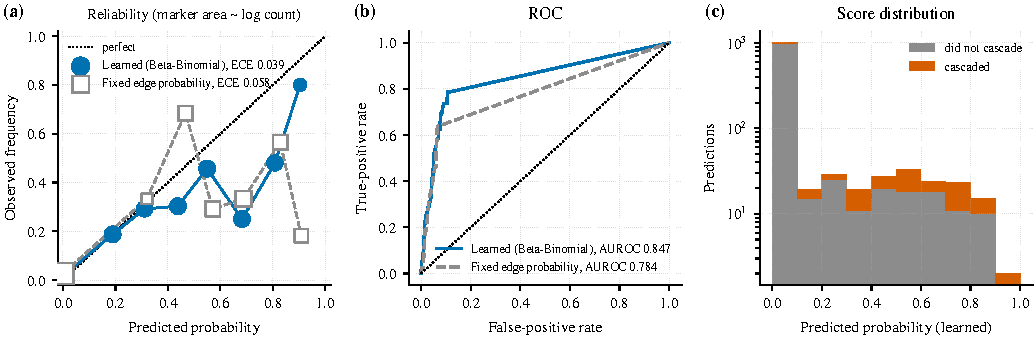
\includegraphics[width=0.98\textwidth]{fig_calibration.pdf}
\caption{Who-is-next prediction on the synthetic held-out set. (a) Reliability diagram. (b) ROC curves. (c) Distribution of the learned probabilities.}
\end{figure}

\begin{simplebox}
A good prediction has two properties. It should \emph{rank} well (the services that really fall are among the highest). And it should be \emph{honest about its numbers} (when it says 70\%, about 70\% of those services really fall). The second property is called \emph{calibration}. Our learned model ranks only slightly better than a fixed-probability version, but it is clearly \emph{better calibrated}: its percentages mean what they say.
\end{simplebox}

\begin{techbox}
On the synthetic held-out set (163 faults, 1\,289 predictions, 69 cascades) the learned propagation model reaches AUROC 0.841 against 0.827 for the same noisy-OR with every edge fixed at 0.7, a Brier score of 0.047 against 0.052 and an expected calibration error of 0.033 against 0.051. The reliability curve is noisy in the upper bins, which hold few predictions. Brier score $=\frac1n\sum_i(p_i-y_i)^2$; ECE $=\sum_b\frac{n_b}{n}\lvert\bar p_b-\bar y_b\rvert$ over equal-width bins.
\end{techbox}

\begin{warnbox}
On the \emph{real} systems this experiment cannot be done well: only 10 of 535 predictions were followed by a cascade, because real faults are mostly single-service outages that the systems absorb. The real-system comparison (AUROC 0.742 against 0.633) is not informative. Never say ``learned cascade prediction works on real systems''. Say ``it is better calibrated on synthetic cascades, and real cascades were too rare for a real-system test''.
\end{warnbox}

\begin{saybox}
``Noisy-OR is the independent-cascade model. Our contribution is learning the edge probabilities online as Beta--Binomial posteriors from the system's own incidents. Calibration is better than fixed probabilities (ECE 0.033 against 0.051); ranking is only slightly better; and on real systems cascades were too rare to test it.''
\end{saybox}
